\documentclass[10pt,a4paper]{article}
\usepackage[utf8]{inputenc}
\usepackage[english]{babel}
\usepackage{amsmath}
\usepackage{amsfonts}
\usepackage{amssymb}
\usepackage{graphicx}
\usepackage{todonotes}
\usepackage{listings}             % Include the listings-package

\usepackage[left=2cm,right=2cm,top=2cm,bottom=2cm]{geometry}

\begin{document}
%%%%%%%%%%%%%%%%%%%%%%%%%%%%%%%%%%%%%%%%%%%%%%%%%%%%%%%%%%%%%%%%%%%%%%%%%%%%%%%
%\vspace*{\stretch{1.0}}
\begin{center}
\Large\textbf{Report 3: Recurrent neural networks}\\
\large Author: \textit{Jannes Nys}
\end{center}
%\vspace*{\stretch{2.0}}
%%%%%%%%%%%%%%%%%%%%%%%%%%%%%%%%%%%%%%%%%%%%%%%%%%%%%%%%%%%%%%%%%%%%%%%%%%%%%%%


\section{Hopfield network for digit reconstruction}
In this section, we use a Hopfield network to reconstruct $15 \times 16$ pixel digits. Since $p/N = 10/240$ is small, the probability of instability is small.

\begin{figure}[htb]
\centering
\begin{minipage}{0.08\textwidth}

\includegraphics[width=\textwidth]{figs/attractors.png}
\end{minipage}%
\begin{minipage}{0.08\textwidth}
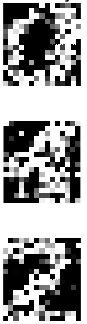
\includegraphics[width=\textwidth]{figs/noisy_digits.png}
\end{minipage}%
\begin{minipage}{0.08\textwidth}

\includegraphics[width=\textwidth]{figs/partially_reconstructed.png}
\end{minipage}%
\begin{minipage}{0.08\textwidth}

\includegraphics[width=\textwidth]{figs/reconstructed.png}
\end{minipage}%
\caption{From left to right: attractor states, noisy digits, reconstructed digits after 1 iteration, reconstructed digits.}
\end{figure}

The retrieval states are the attractors of the system. They form the local minima of the associated energy function of the system. By distorting the original image (which is located at a local minimum), one increases the temperature of the system, allowing for a jump to a state (image) away from the original minimum. The higher the noise level, the less the distorted image resembles the original image. The Hopfield network is used to `cool the system down', lowering the energy along the gedesics defined by the weight matrix, such that it reaches a local minimum. This minimum can of course be different from the original one if distorting the image results in an image located in another mode of the energy surface. In the following, we use the term `distortion energy', which is the analogous of `thermal energy'. It refers to the average energy difference that can is added to an image in a ground state by distortion. 

When the noise level is low, the distorted image ends up within a small perimeter around the original image. Hence, in the majority of the cases, the image is properly restored.
When the temperature increases, the contour of the domain of distorted images increases in energy. The first false image reconstructions occur when the distortion energy reaches the same energy as the ridge between its original minimum and another local minimum. In this case, when the distorted image is cooled down, it may end up in the wrong minimum. Hence, if this local-minima-separating ridge has a small energy, then this phenomenon will occur at low distortion.  For a noise fraction between $0$ and $1$, I observed no false reconstructions. However, if I increase the noise level above $1$, more interesting cases occur. The digits for which we first observe a false reconstruction when increasing the noise level, is at distortion level\footnote{The noise distortion level of the \texttt{hopdigit} function is supposed to be a noise fraction. However, nothing prevents us from taking values above 1.} $5$, for the $2$ and $9$. These respectively end up in the $7$ and $2$ minimum a large number of cases.

A second factor that needs to be taken into account is the number of iterations in the cooling process. If the number of iterations is too low, the system will not be able to fully cool down and reach a minimum. The maximum number of iterations should be large enough (such that the image results in an attractor state) and depends on the distortion level: the higher the distortion, the more steps are needed to guide the system to a local minimum. For the case at hand, $100$ iterations is generally sufficient.\\

A problem of Hopfield networks is that spurious states may occur. These attractors are states which are not put in explicitly, but are generated from a linear combination of retrieval states. In the digit reconstruction, I did not find such states in any simulation (even when the noise level is high). The reason for this is that it is unlikely to reach such a state, since it forms a perfect symmetry. When the number of iterations is kept low, one can recognize combinations of digits in the reconstructed images. These states are close to the spurious states. For discrete pixel values (e.g.\ black-white instead of the current gray scale), these spurious states would form a bigger problem. This is the case when the output transfer function \texttt{purelin} is changed to \texttt{sign} in the Hopfield network.

As a final test, I used other handwritten versions of the digits. These are also included in the \texttt{digits} workspace. Even with a low noise input, the Hopfield network can propagate to the wrong attractor state.

\section{Elman recurrent network approximation for the Hammerstein function}
I first adapted the \texttt{elmants2} script. In the original version, the division of the data into training and test set occurs twice: once manually, once automatically. Therefore, we include the following code before training (avoiding automatic division):
\lstset{language=Matlab}          % Set your language (you can change the language for each code-block optionally)
\begin{lstlisting}
net.divideFcn = 'dividetrain';
\end{lstlisting}
In this parameter state, the network assigns all targets to the training set and no targets to either the validation or test sets. Hence, all of the \texttt{n\_tr} training set entries are now effectively used in the training process.

In the documentation of \texttt{newelm}, \texttt{Matlab} makes the following interesting warning:
\begin{quote}
\textit{``Algorithms which take large step sizes, such as TRAINLM,
     and TRAINRP, etc., are not recommended for Elman networks.  Because
     of the delays in Elman networks the gradient of performance used
     by these algorithms is only approximated making learning difficult
     for large step algorithms."}
\end{quote}

\begin{figure}[tbh]
\centering
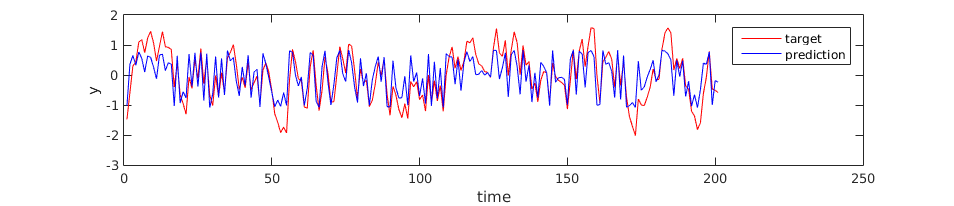
\includegraphics[width=\textwidth]{figs/tansig_purelin.png}
\caption{Output of an Elman network with $10$ neurons in the hidden layer and the \texttt{tansig} and \texttt{purelin} transfer function in the hidden and output layer respectively. The correlation between both data sets is $0.7994$. \label{fig:tansig_purelin}}
\end{figure}

In contrast to the non-dynamical case, where \texttt{trainlm} is often the default learning algorithm, \texttt{newelm} uses \texttt{traingdx} by default. This algorithm uses a gradient descent with momentum and adaptive learning rate back propagation.

The use of the \texttt{logsig} transfer function is to be avoided, since it since its output domain is strictly positive. Especially when used in the output layer, the performance is low.

Even with the most simple architecture with \texttt{purelin} in the hidden and output layer, strong correlations $>0.75$ between the prediction and target test set are obtained\footnote{In the following, we will refer to this correlation as `the correlation of the test set'. We opt to quantify the performance of a network on the test set by this correlation, since the underlying Hammerstein function models a stochastic process.}. Using the \texttt{tansig} transfer function in the hidden layer efficiently yields large correlations in the test set. However, it does not properly reproduce the outliers. This is illustrated in Fig.~\ref{fig:tansig_purelin}. However, we choose this configuration as the optimal one, since the test set correlation is maximal compared to all tested configuration.

\begin{figure}[tbh]
\centering
\begin{minipage}{0.4\textwidth}
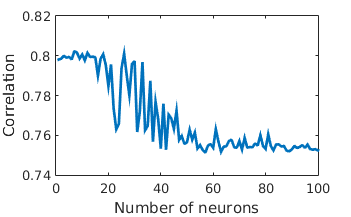
\includegraphics[height=3cm]{figs/correlation_map.png}
\end{minipage}%
\begin{minipage}{0.4\textwidth}
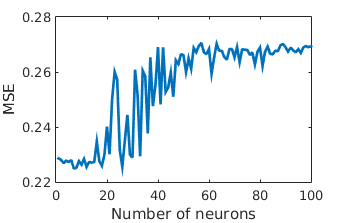
\includegraphics[height=3cm]{figs/mse_map.png}
\end{minipage}%
\caption{Correlation (left) and mean-square error (right) of the Elman network tested on the test set in function of the number of neurons in the hidden layer. \label{fig:elman}}
\end{figure}

In Fig.~\ref{fig:elman} we map the test-set correlation and MSE in function of the number of neurons in the hidden layer. From this plot, it is clear that the number of neurons must be limited to $< 20$ in order for the network to be generalizable.





\end{document}